%...oooOOO000OOOooo......oooOOO000OOOooo......oooOOO000OOOooo...
% This example is protected under GPL2+ License
% This is a basic show example for the OLReport package.
% Jimmy Aguilar Mena. August, 2015
% Any bug report, or comment: kratsbinovish@gmail.com
% If you use this package, please inform to the author if possible
% via e-mail.
%...oooOOO000OOOooo......oooOOO000OOOooo......oooOOO000OOOooo...

\documentclass[11pt]{report}
\usepackage{OLReport}

\title{This is the title, it can be relatively long, just try.}
\author{Myname Lastname}
\supervisor{First Supervisor\newline Secound Supervisor}

\begin{document}
\maketitle
\begin{specification}
	This are the specifications bla bla bla
\end{specification}

\begin{abstract}
	This is the abstract remember this will not have numbers.
\end{abstract}

\tableofcontents
\newpage

\section{Introduction}
This is my very long introduction This is my very long introduction This is my very long introduction This is my very long introduction This is my very long introduction This is my very long introduction 

\section{This is a new section}
Here the text and the numeration is as usual in the original template the introduction is numerated.

\section{Another seccion}
Another section text

\subsection{My subseccion}
Subsection text

\subsubsection{Now a subsubseccion}
Subsubsection text in third level of numeration. After this level there are not numbers

\begin{figure}[h]
	\centering
	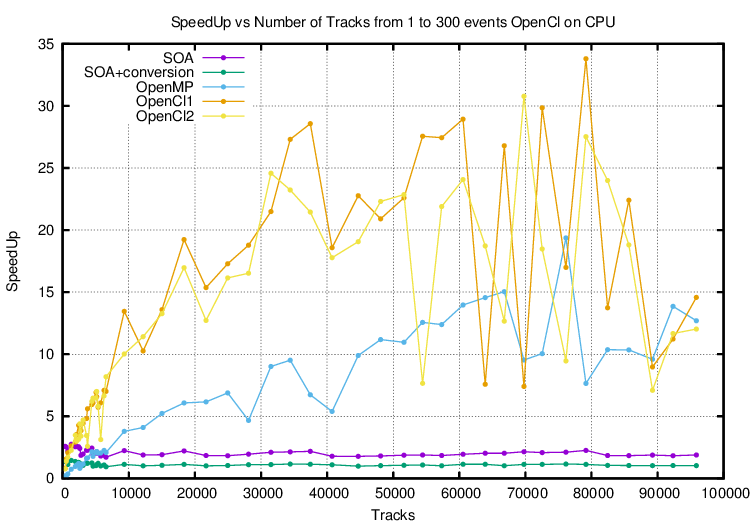
\includegraphics[width=0.7\textwidth]{SU_OMP_Code}
	\caption{This is a figure}
\end{figure}

\begin{table}[h]
	\centering
	\begin{tabular}{|c|c|c|c|c|}
		\hline  &  &  &  &  \\ 
		\hline  &  &  &  &  \\ 
		\hline  &  &  &  &  \\ 
		\hline 
	\end{tabular} 
	\caption{This is a table}
\end{table}


If you add some bibliography use numbered chapter name too. Please complains or problems just inform or solve and contribute :)
\end{document}          
